\section{Estudo de Caso}
Esse estudo de caso apresenta uma análise exploratória de uma base de dados do IMDB\footnote{\url{https://www.kaggle.com/carolzhangdc/predict-imdb-score-with-data-mining-algorithms/data}}, retirada do Kaggle\footnote{\url{https://www.kaggle.com/}}, que é uma ferramenta de competições e aprendizado online de ciência de dados, e serão aplicados modelos de aprendizado de máquina para tentar prever, com o menor erro possível, a nota dos filmes. Nessa análise, serão retiradas observações que podem auxiliar na criação do modelo de aprendizado.

Essa base de dados, a \textit{MDB 5000 Movie Dataset}, foi adquirida de forma gratuita no Kaggle, ela nunca foi utilizada em competições. Esses dados contém informações de cerca de 5000 filmes retirados do IMDB e apresenta informações como lucro, investimento, quem dirigiu, o ano em que foi publicado, atores e atrizes principais, duração etc.
\subsection{Analise Exploratória}
A tabela 2 contém todas as colunas que existem na base de dados. Um total de 28 colunas numéricas e de texto e 5093 registros. A maioria dos dados tem uma porcentagem de dados faltantes abaixo de 1\%, mas outros, como \textbf{director\_name}, \textbf{plot\_keywords} têm mais de 2\% e a coluna de lucro (\textit{gross}) possui 17.5\%, o que pode atrapalhar um pouco no processo, mas isso ainda não pode ser dito com certeza
\newcolumntype{L}{>{\raggedright\arraybackslash}m{5cm}}
\begin{longtable}{|l|l|L|c|}
\caption{ Colunas do Dataset }
\\ \hline
\textbf{Coluna}              & \textbf{Tipo} & \textbf{Descrição}                      & \textbf{Dados Faltantes} \\ \hline
color                        & String        & Filme é em preto e branco ou colorido   & 0.4\%                    \\ \hline
director\_name               & String        & Nome de quem dirigiu                    & 2.1\%                    \\ \hline
num\_critic\_for\_reviews    & Integer       &                                         & 1\%                      \\ \hline
duration                     & Number        & Duração do filme                        & 0.32\%                   \\ \hline
director\_facebook\_likes    & Number        & Total de likes da pessoa diretora       & 2.1\%                    \\ \hline
actor\_3\_facebook\_likes    & Number        & Total de likes terceira atriz principal & 0.5\%                    \\ \hline
actor\_2\_name               & String        & Nome da segunda atriz principal         & 0.3\%                    \\ \hline
actor\_1\_facebook\_likes    & Number        & Total de likes da primeira atriz        & 0.1\%                    \\ \hline
gross                        & Number        & Lucro do filme                          & 17.5\%                   \\ \hline
genres                       & String        & Gêneros do filme                        & 0\%                      \\ \hline
actor\_1\_name               & String        & Nome da primeira atriz principal        & 0.1\%                    \\ \hline
movie\_title                 & String        & Título do filme                         & 0\%                      \\ \hline
num\_voted\_users            & Integer       & Número de usuários que votaram          & 0\%                      \\ \hline
cast\_total\_facebook\_likes & Integer       & Total de likes do elenco                &                          \\ \hline
actor\_3\_name               & String        & Nome terceira atriz principal           & 0.5\%                    \\ \hline
facenumber\_in\_poster       & Number        & Número de rostos no poster do filme     & 0.3\%                    \\ \hline
plot\_keywords               & String        & Palavras-chave do enredo                & 3\%                      \\ \hline
movie\_imdb\_link            & String        & Link do filme no IMDB                   & 0\%                      \\ \hline
num\_user\_for\_reviews      & Number        & Número de usuários que fizeram review   & 0.4\%                    \\ \hline
language                     & String        & Língua em que o filme foi distribuído   & 0.2\%                    \\ \hline
country                      & String        & País de origem do filme                 & 0.1\%                    \\ \hline
content\_rating              & String        & Classificação indicativa                & 6\%                      \\ \hline
budget                       & Number        & Orçamento                               & 9.8\%                    \\ \hline
title\_year                  & Number        & Ano de lançamento                       & 2.1\%                    \\ \hline
actor\_2\_facebook\_likes    & Number        & Total de likes Segunda atriz principal  & 0.3\%                    \\ \hline
imdb\_score                  & Number        & Nota no IMDB                            & 0\%                      \\ \hline
aspect\_ratio                & Number        & proporção da tela                       & 6.5\%                    \\ \hline
movie\_facebook\_likes       & Number        & Total de likes do filme              & 0\%                      \\ \hline
\end{longtable}


Uma análise foi realizada com \textbf{Python}\footnote{Todos os arquivos gerados podem ser encontrados em \url{https://github.com/gabriel-ma/TCC}} e as bibliotecas \textbf{pandas}\footnote{https://pandas.pydata.org/}, \textbf{matplotlib}\footnote{https://matplotlib.org/} e \textbf{seaborn}\footnote{https://seaborn.pydata.org/}. Inicialmente os dados foram importados e uma análise geral foi realizada com o \textbf{pandas profiling}\footnote{https://github.com/pandas-profiling/pandas-profiling} e observações iniciais foram feitas:
\begin{itemize}
    \item 15 colunas contém dados numéricos;
    \item 12 são dados categóricos;
    \item Existem filmes de cerca de 65 países;
    \item Existem 45 dados duplicados;
    \item O ator que mais participou dos filmes é o Robert De Niro;
    \item A maior parte dos filmes é colorida;
    \item 3808  filmes foram feitos nos Estados Unidos;
    \item O lucro médio dos filmes é de \$48.468.000,00;
    \item O filme com a maior nota tem 9.5;
    \item O filme com a menor nota tem 1.6;
    \item A nota média dos filmes é de 6.44;
    \item O orçamento médio dos filmes é de \$39.753.000,00;
    \item 4662 filmes estão disponíveis em inglês;
    \item O filme com o maior número de críticas tem 813 críticas;
    \item Com 258, 2009 é o ano com a maior quantidade de filmes nos dados;
    \item A coluna \textbf{cast\_total\_facebook\_likes} tem uma correlação muito alta\\ com \textbf{actor\_1\_facebook\_likes}.
\end{itemize}

Uma hipótese que pode logo levantada é de que os dados estão enviesados. De acordo com o item 10, cerca de 3808 filmes foram feitos nos Estados Unidos, o que faz com que ao treinar o modelo a partir desses dados, o algoritmo pode ser ótimo para prever, por exemplo, notas de filmes norte-americanos, mas péssimo para prever filmes sul-americanos.

\begin{figure}[H]
\centering
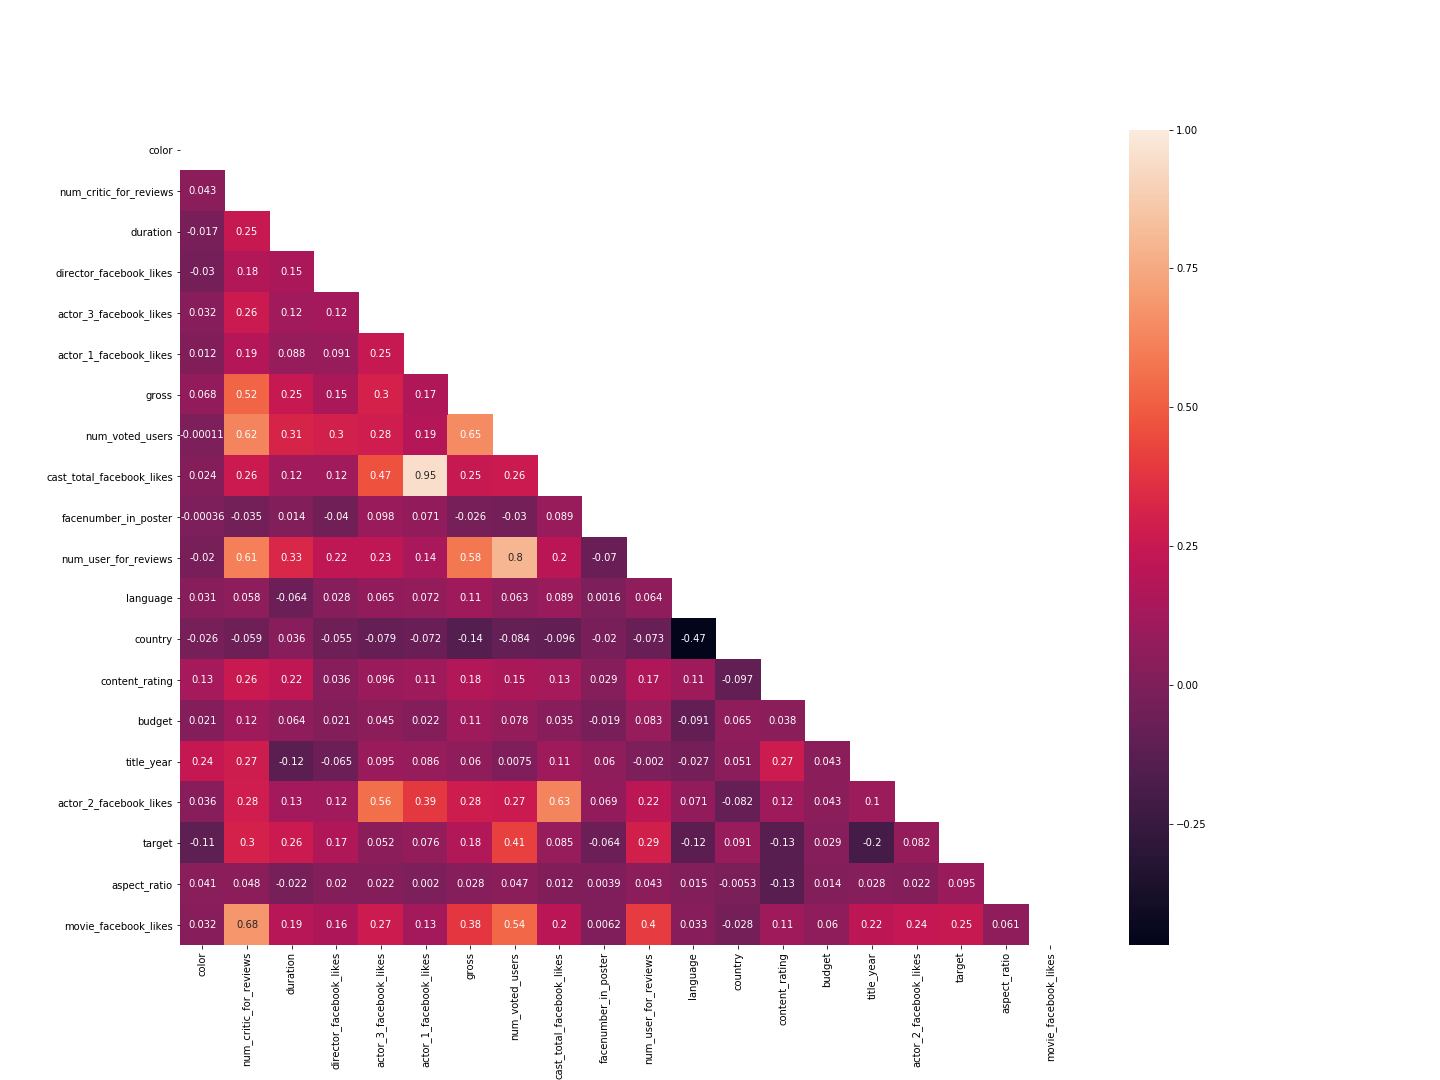
\includegraphics[height=15cm]{imagens/heatmap.png}
\caption{Heatmap}
\label{heatmap}
\end{figure}

A figura \ref{heatmap} representa um \textit{heatmap} (mapa de calor) que mostra o quanto os campos estão correlacionados. Por exemplo, se um campo \textbf{x} tem uma correlação positiva muito alta com o campo \textbf{y}, isso significa que quando o valor de um aumentar, o valor do segundo campo provavelmente também irá aumentar. Na figura acima, é possível notar que quanto maior a relação entre dois campos, mais claro o quadrado que exibe a relação fica no mapa. 
Na mesma figura é possível ver que existem campos com uma correlação maior com a nota (\textit{target}) como \textbf{num\_crit\_for\_reviews} e \textbf{num\_voted\_users}. 

É possível assumir que algumas colunas não são necessárias para a análise, como \textbf{imdb\_link}, que é apenas o \textit{link} do filme na página do IMDB e não tem relação nenhuma com a nota.

Alguns gráficos foram gerados para poder realizar uma análise mais profunda dos dados: 

\begin{figure}[H]
\centering
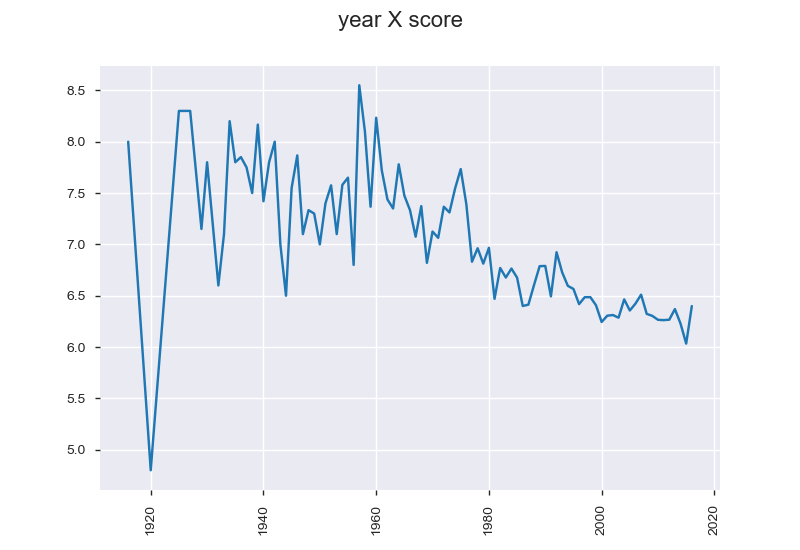
\includegraphics[height=10cm]{imagens/yearXscore.png}
\caption{Ano X Nota}
\label{yearXscore}
\end{figure}

Na figura \ref{yearXscore} é possível perceber que a média das notas veio caindo. Excetuando o ano de 1920, que teve uma média incrivelmente baixa, os anos seguintes se mantiveram entre 8.5 e 6.5. A partir da década de 80, o cenário começou a mudar e as médias começaram a baixar, chegando em 2016 (último ano que existe no \textit{dataset}) a aproximadamente 6.5.

\begin{figure}[H]
\centering
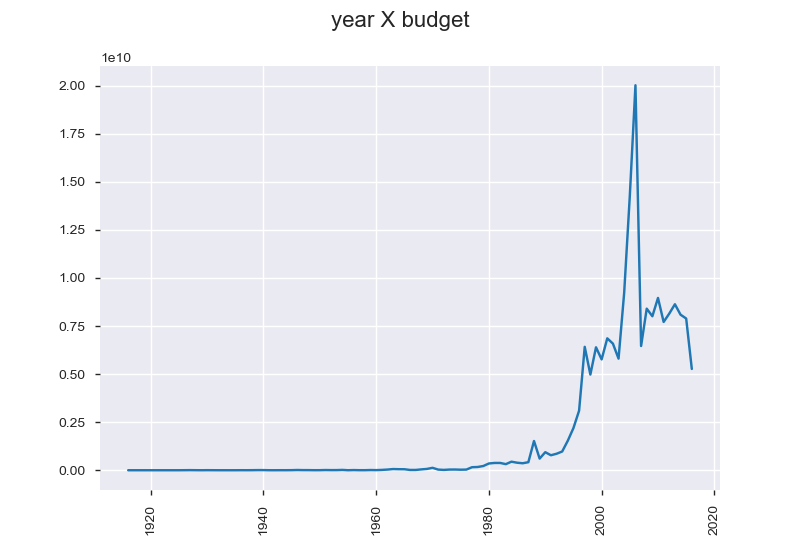
\includegraphics[height=10cm]{imagens/yearXbudget.png}
\caption{Investimento X Ano}
\label{budgetXyear}
\end{figure}
A figura \ref{budgetXyear} acima mostra que o investimento nos filmes aumentou consideravelmente. Entre a década de 90 e os anos 2000 teve um aumento quase exponencial.

\begin{figure}[H]
\centering
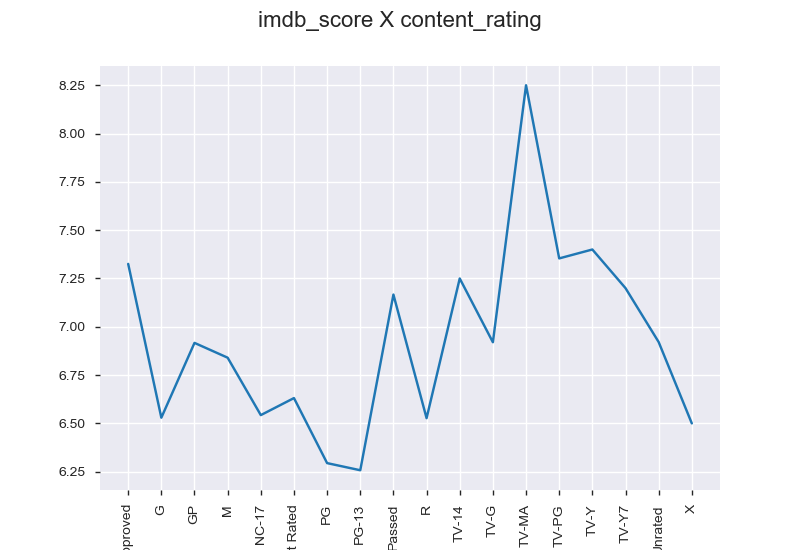
\includegraphics[height=10cm]{imagens/scoreXcontent.png}
\caption{Classificação indicativa X Nota}
\label{ratingXscore}
\end{figure}
Outra variável que pode influenciar a nota dos filmes é a classificação indicativa. A figura \ref{ratingXscore} mostra que filmes com a classificação \textbf{TV-MA} tendem a ter uma nota maior. Cerca de 2098 amostras encontradas nesses dados contêm a classificação \textbf{R}, porém a média das notas para esses filmes é de pouco mais de 6.5.

\subsection{Extract}
No primeiro passo do ETL, que é o de extração, \textit{extract}, os dados foram extraídos com auxilio do \pdi com um \textit{step} de \textit{read csv}, já que o arquivo é um csv. Existiu a necessidade de formatar corretamente os campos de números, e nos de texto foi necessário realizar uma operação \textit{trim} para remover espaços em brancos desnecessários. 

\subsection{Transform}
No segundo passo do ETL, o de transformação, \textit{transform}, foram usados passos para substituir alguns valores nulos, como, por exemplo, no campo \textbf{color}, os dados que não eram preenchidos eram substituídos por 0. 

Com o auxílio da linguagem \textbf{Python} com as bibliotecas \textbf{pandas}, \textbf{sklearn}\footnote{https://scikit-learn.org/stable/} e \textbf{numpy}\footnote{http://www.numpy.org/} através do \textbf{Jupyter Notebook}\footnote{http://jupyter.org/}, diversos tratamentos adicionais nos dados foram realizados, como preencher valores nulos, que não foram tratados no \pdi pela média, quando necessário. No \pdi se fez necessário adicionado um \textit{step} de \textbf{group by} para tratar campos, substituindo o seu valor (quando faltante) pela média ou pela mediana. 

Outros \textit{steps} foram usados para fazer um mapeamento dos dados, por exemplo, a coluna \textbf{director\_name} do jeito que está originalmente não iria ser muito útil na análise, pois os algoritmos de regressão aplicados não conseguem trabalhar com campos de texto. Para isso, esses dados foram substituídos por números que identificam o diretor do filme. O mesmo aconteceu com as colunas \textbf{color}, \textbf{language}, \textbf{country}, \textbf{content\_rating} e as colunas de atores. Manter essas colunas como texto iria atrapalhar a análise, já que vários dos algoritmos usados não conseguem trabalhar com campos de texto. A figura \ref{pentahoTransformation} mostra todos os \textit{steps} que foram criados para o processo de ETL no \pdi.

\begin{figure}[H]
\centering
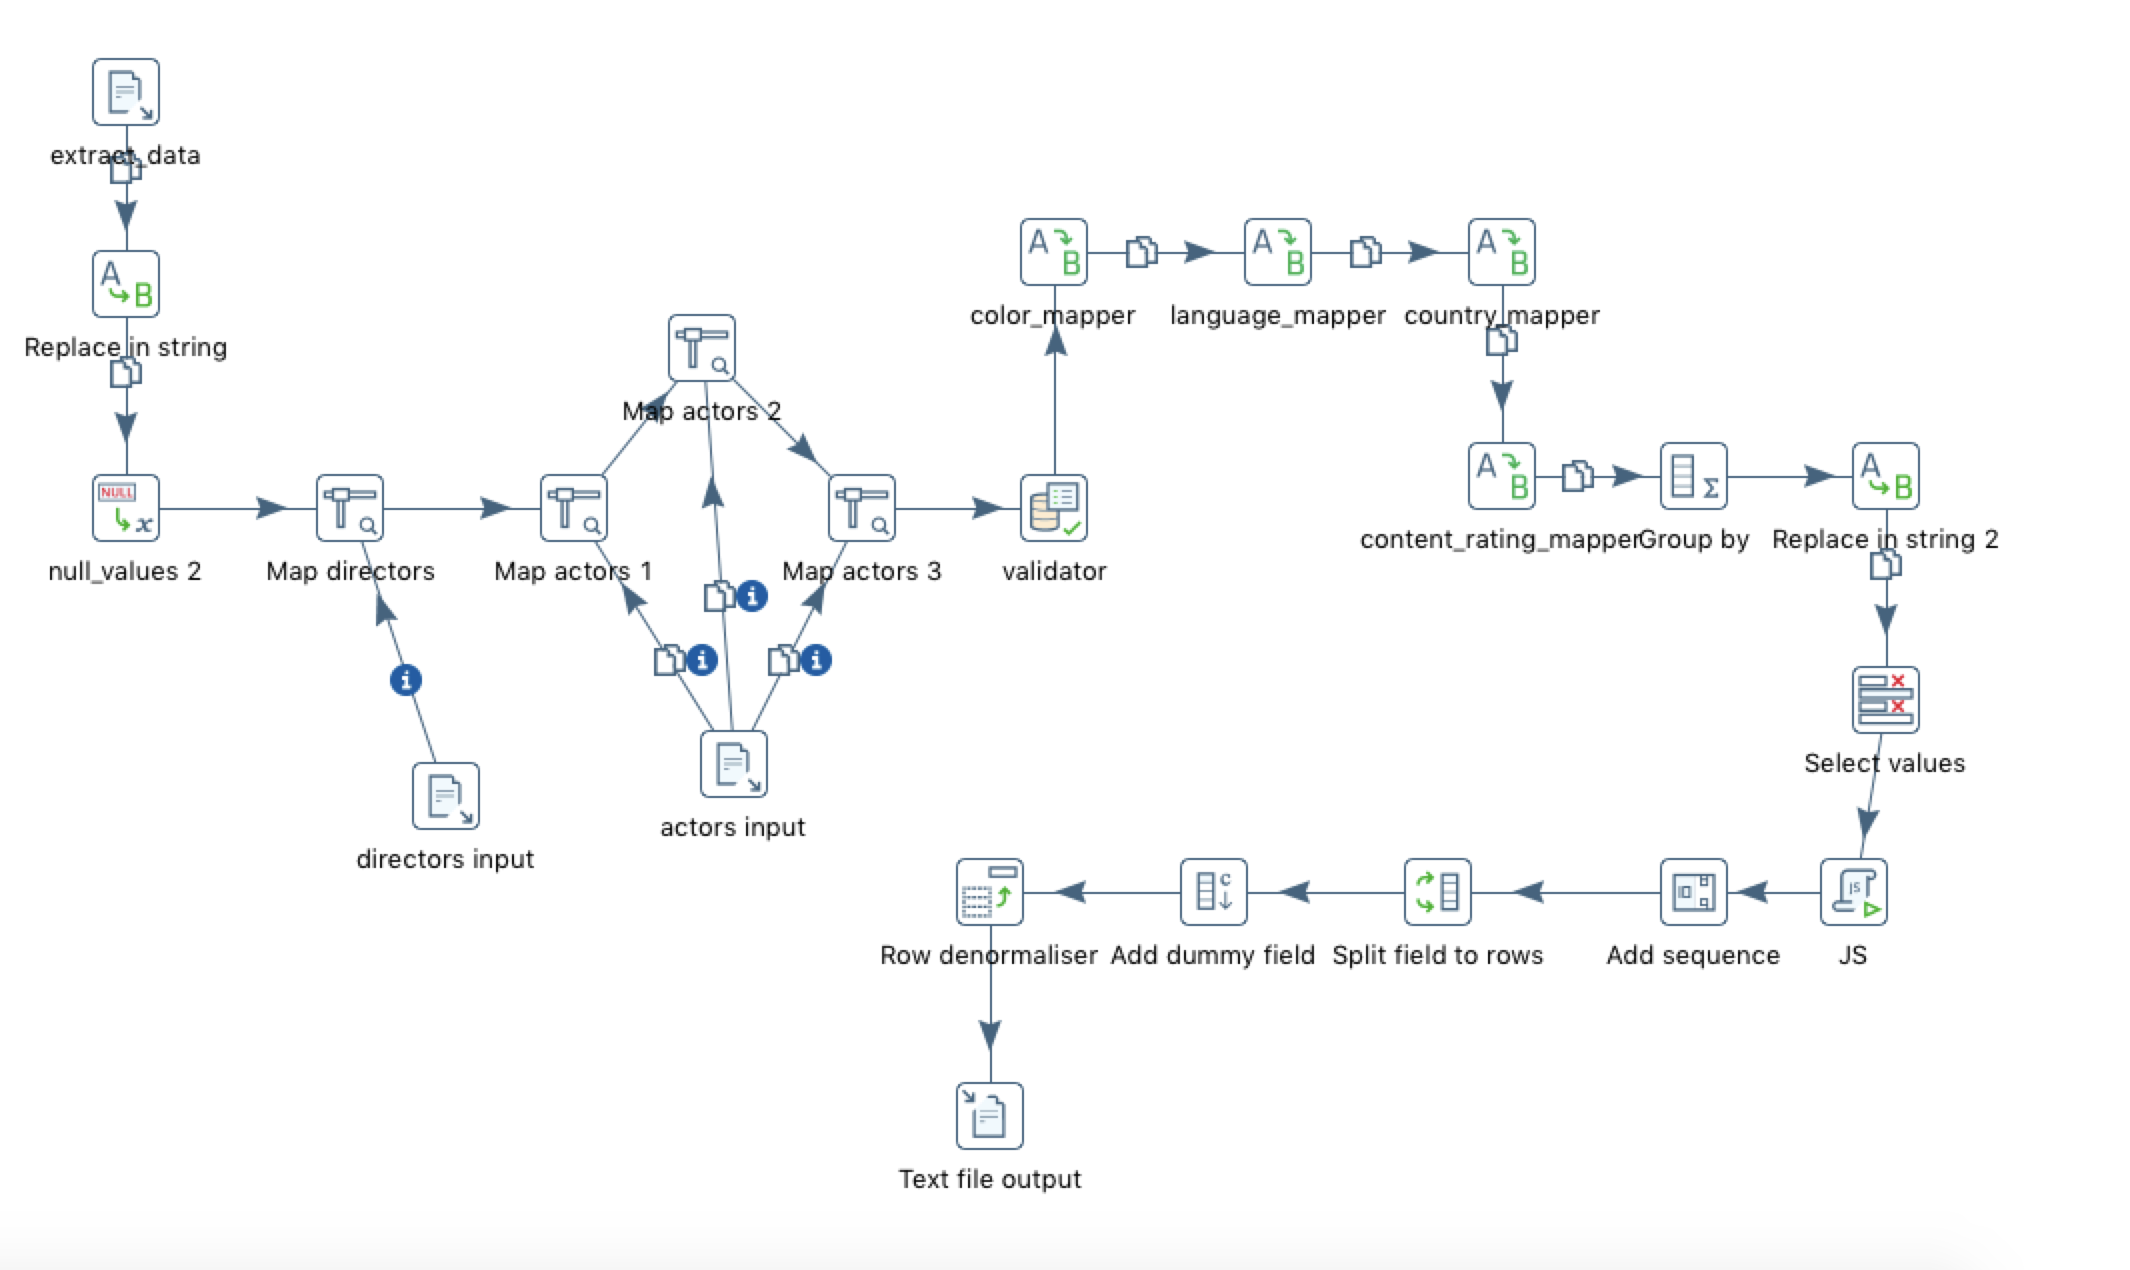
\includegraphics[height=6cm, width=9cm]{imagens/transformacao.png}
\caption{Processo do pentaho}
\label{pentahoTransformation}
\end{figure}

Algumas colunas novas foram geradas e essas são derivadas de colunas existentes, como \textbf{plot\_keywords\_num}. Tiveram \textit{steps} responsáveis por fazer uma transformação na coluna \textbf{genres}, transformando cada valor em uma coluna e se o filme conter o gênero da coluna, ela é marcada com 1, senão, 0, como mostra a figura \ref{newcolumns}.

\begin{figure}[H]
\centering
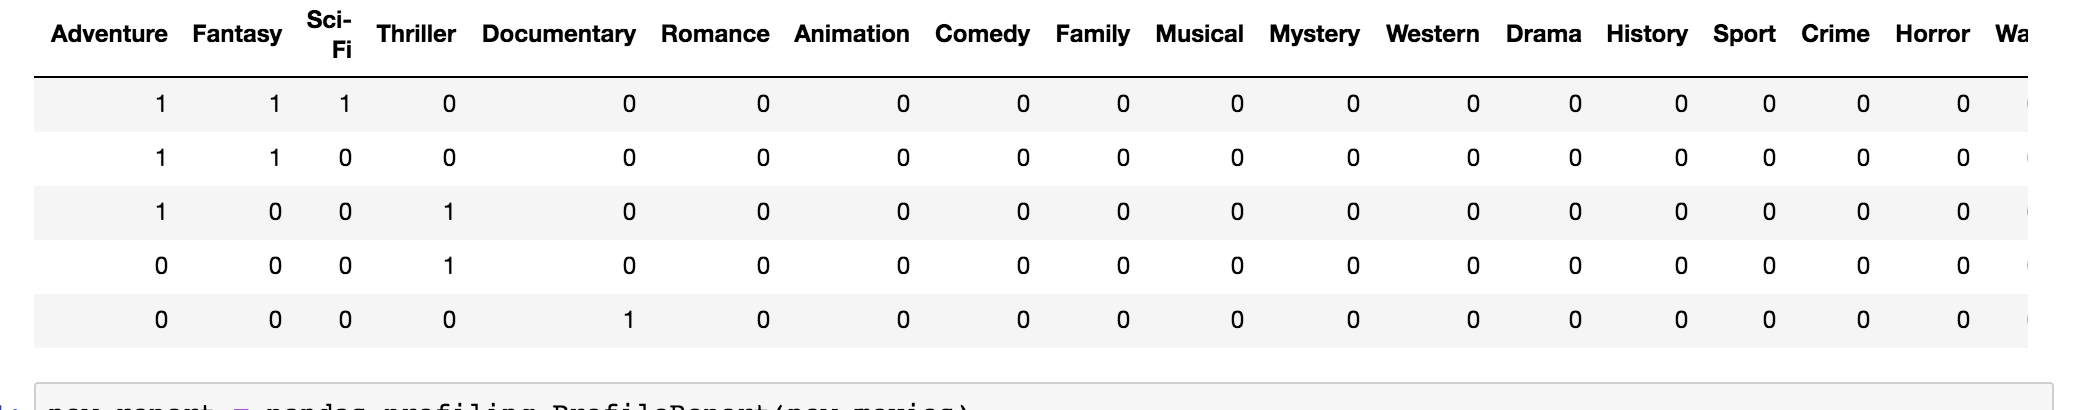
\includegraphics[height=3cm]{imagens/genres.png}
\caption{Novas colunas de gênero}
\label{newcolumns}
\end{figure}

\subsection{Load}
O último passo, que é o carregar, \textit{load}, apenas carregou os dados em um outro arquivo csv, com o \textit{step text file output}. Esse arquivo é usado mais tarde no WEKA.

\subsection{Hipóteses}
A hipótese principal é se seria possível prever a nota de um filme com base nos dados disponíveis e qual o nível de precisão.

Além disso, como dito anteriormente, outra hipótese que pode ser levantada é a de que os dados estão enviesados, já que contêm muitos filmes feitos nos Estados Unidos. Uma outra que pode ser levada em consideração é se o diretor do filme tem grande influência sobre a nota dele. Também é possível verificar o quanto a nota do filme vai influenciar no lucro dele e o quanto o investimento feito pode influenciar a nota.

Após todos os passos acima, o próximo é realizar o processo de \textit{machine learning}, levando em consideração todos as hipóteses levantadas. Os dados foram carregados no WEKA e algoritmos de aprendizado de máquina foram usados. Um segundo \textit{dataset}, sem os filmes norte-americanos, foi criado e também carregado no WEKA, para validar ou não a afirmação feita de que os dados estão enviesados. 

Em resumo:

\begin{itemize}
    \item Prever nota de um filme com base nos dados disponíveis;
    \item A grande quantidade de filmes dos EUA adiciona um viés nos dados;
    \item Influência do investimento na nota;
    \item Influência do país na nota;
    \item Influência do diretor na nota;
\end{itemize}

\subsubsection{Resultados}
As análises realizadas levaram em conta o RMSE, \textit{root mean squared error}, que calcula a raiz da diferença entre valor previsto e o valor real, como mostra a formula abaixo:

$RMSE = \sqrt{\frac{1}{n}\Sigma_{i=1}^{n}{\Big({predicted-actual}\Big)^2}}$
 
O MSE é muito usado em vários algoritmos porque ele tende a ser a medida mais fácil de ser manipulada matematicamente.

Em um primeiro momento, os dados gerados a partir do \pdi e as bibliotecas do \textit{Python} foram usados para selecionar o algoritmo de predição com os melhores resultados. Para isso, foram realizadas diversas análises com esses algoritmos no WEKA: os que tiveram o menor RMSE, tanto método de \textit{cross-validation} e o de 70\% split, foram \textit{linear regression}, \textit{bagging}, \textit{random committee} e \textit{random forest}, como mostra as tabelas abaixo:

\begin{longtable}{|l|l|l|}
\caption{Resultados da previsão usando \textit{cross-validation}}
\label{cvfull}
\\ \hline
\textbf{Algoritmo} & \textbf{RMSE}  \\ \hline
Linear Regression      & 0.827                    \\ \hline
Bagging                & 0.7685                   \\ \hline
Random Committee       & 0.7754                   \\ \hline
Random Forest          & 0.774                    \\ \hline
\end{longtable}


\begin{longtable}{|l|l|l|}
\caption{Resultados da previsão usando 70\% para treinamento e 30\% para teste}
\label{splitfull}
\\\hline
\textbf{Algoritmo} & \textbf{RMSE} \\ \hline
Linear Regression      & 0.8122                   \\ \hline
Bagging                & 0.7529                   \\ \hline
Random Committee       & 0.7468                   \\ \hline
Random Forest          & 0.7245                   \\ \hline
\end{longtable}



Para testar a hipótese de que a grande quantidade de filmes dos EUA adiciona um viés nos dados, os filmes feitos nos Estados Unidos foram removidos do \textit{dataset}. Ao remover esses filmes e também aplicar o algoritmo que teve os melhores resultados, o \textit{random forest}, ele retornou um RMSE de 0.7674 (figura \ref{nousacv}) com o método \textit{cross-fold validation} e 0.7341 (figura \ref{nousasplit}) usando o \textit{percentage split}. Os resultados não mudaram tanto, porém a quantidade de amostras sim, foram de 4998 para 1224. Talvez o filme ser do EUA tenha de fato influência sobre a nota final, porém não é possível definir com clareza somente com essa quantidade de dados, já que muita informação se perde.

\begin{figure}[H]
\centering
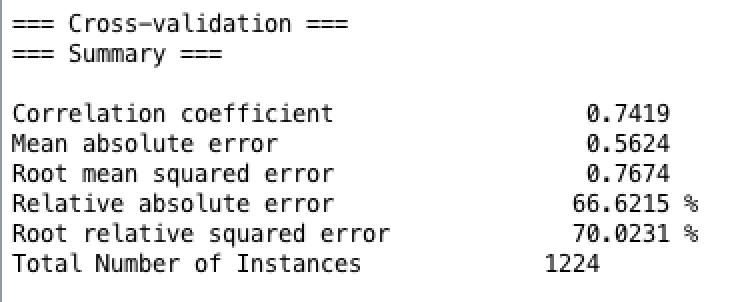
\includegraphics[height=5cm]{imagens/sem_usa_cv.png}
\caption{Sem filmes dos EUA e usando \textit{cross-validation}}
\label{nousacv}
\end{figure}

\begin{figure}[H]
\centering
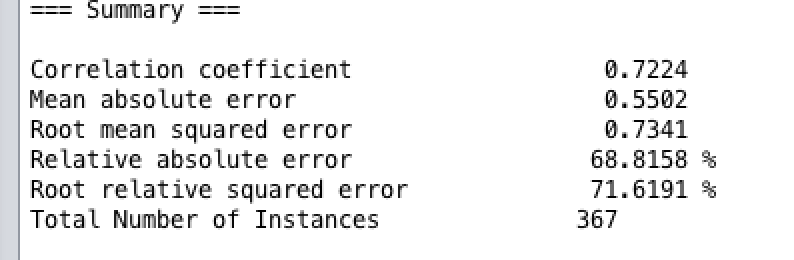
\includegraphics[height=5cm]{imagens/sem_usa_split.png}
\caption{Sem filmes dos EUA e usando \textit{percentage split}}
\label{nousasplit}
\end{figure}


Em seguida, a outra hipótese levantada é de que o investimento feito no filme tem influência na nota final. A figura \ref{nobudgetcv} mostra um RMSE de 0.7496, utilizando \textit{cross-validation} e a figura \ref{nobudgetsplit} mostra um erro de 0.7235. Mesmo o RMSE sendo um pouco menor, a diferença no erro entre os resultados obtidos nessa avaliação e com todos os dados, também é pequena demais para poder ser de alguma significância.

\begin{figure}[H]
\centering
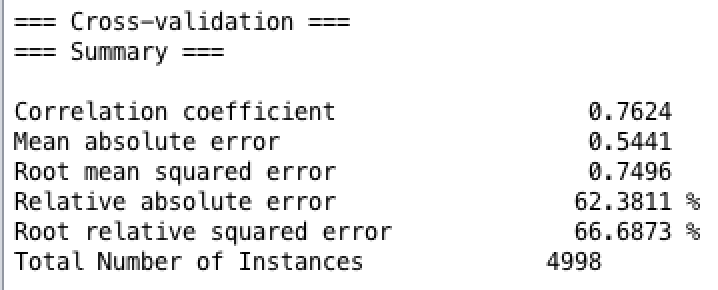
\includegraphics[height=5cm]{imagens/no_budget_cv.png}
\caption{Sem a coluna de orçamento e usando \textit{cross-validation}}
\label{nobudgetcv}
\end{figure}

\begin{figure}[H]
\centering
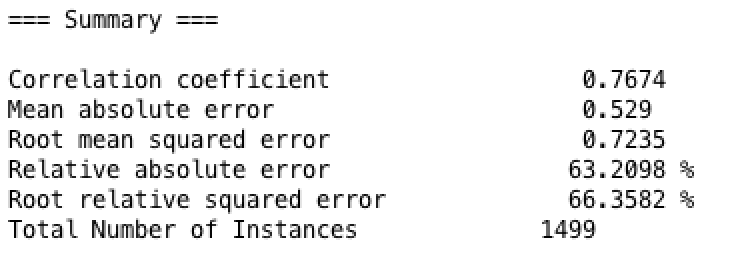
\includegraphics[height=5cm]{imagens/no_budget_split.png}
\caption{Sem a coluna de orçamento e usando \textit{percentage split}}
\label{nobudgetsplit}
\end{figure}


Uma outra hipótese é que o país vai ter influência nos resultados das notas dos filmes. Para testar essa afirmação, a coluna de países foi removida e o mesmo algoritmo citado anteriormente foi usado. A figura \ref{nocountrycv} mostra um RMSE de 0.7462, com \textit{cross validation}. Já a figura \ref{nocountrysplit}, que é com o método \textit{percentage split}, mostra um RMSE de 0.7313. Ao comparar os resultados do \textit{dataset} inteiro, é possível concluir que o país tem sim certa influência na nota, mas é muito pouca para ser significativa. 

\begin{figure}[H]
\centering
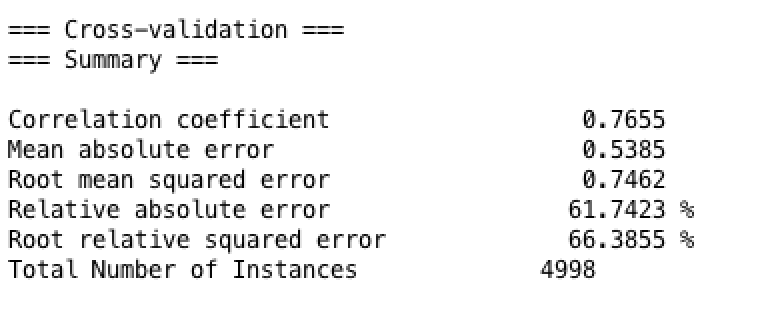
\includegraphics[height=5cm]{imagens/no_country_cv.png}
\caption{Sem a coluna de país e usando \textit{cross-validation}}
\label{nocountrycv}
\end{figure}

\begin{figure}[H]
\centering
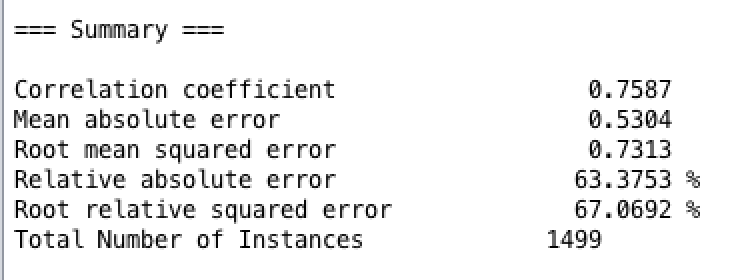
\includegraphics[height=5cm]{imagens/no_country_split.png}
\caption{Sem a coluna de país e usando \textit{percentage split}}
\label{nocountrysplit}
\end{figure}


Por último, a hipótese de que o diretor pode influenciar foi testada. Primeiro, com \textit{cross-validation} como mostra a figura \ref{nodirectorcv} tem um RMSE de 0.7451, já com \textit{percentage split}, tem um erro de 0.7264, como mostra a figura \ref{nodirectorsplit}. Com o método \textit{cross-validation} o erro foi menor, já com a técnica de \textit{percentage split} o RMSE foi um pouco maior, 0.0019. Isso mostra que o diretor escolhido para dirigir o filme não tem tanta influência na nota do filme. 

\begin{figure}[H]
\centering
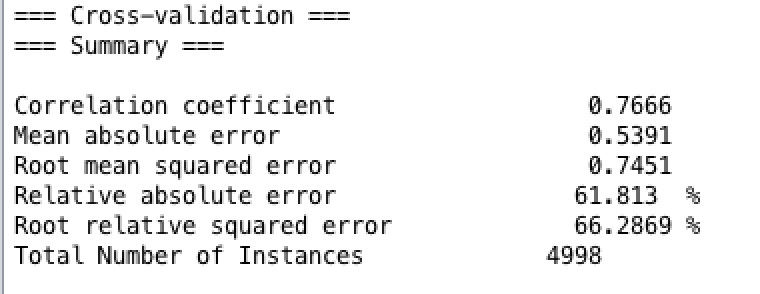
\includegraphics[height=5cm]{imagens/no_director_cv.png}
\caption{Sem a coluna de diretor e usando \textit{cross-validation}}
\label{nodirectorcv}
\end{figure}

\begin{figure}[H]
\centering
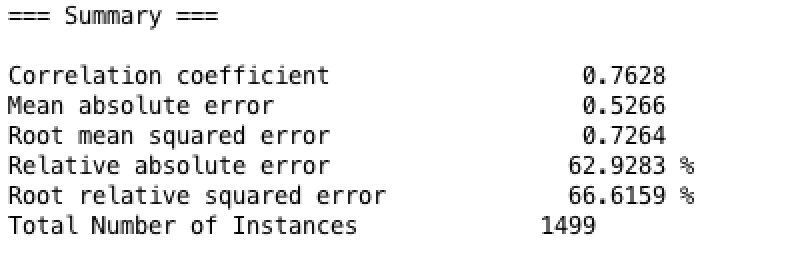
\includegraphics[height=5cm]{imagens/no_director_split.png}
\caption{Sem a coluna de diretor e usando \textit{percentage split}}
\label{nodirectorsplit}
\end{figure}

Dentre todas as hipóteses levantadas, apenas a primeira pôde ser testada com maior precisão, a de prever a nota dos filmes. Utilizando \textit{random forest} e realizando o tratamento dos dados descritos nessa seção, foi possível chegar a um RMSE de 0.7748, com \textit{cross-validation} (tabela \ref{cvfull}) e 0.7245 usando \textit{percentage split} (tabela \ref{splitfull}). 

Diante disso, o trabalho aqui realizado foi capaz de prever as notas com um erro relativamente baixo, de aproximadamente 0.7245, usando \textit{percentage split}. Foi difícil saber com certeza se outros atributos tinham uma influência direta no resultado final, visto que a variação no resultado era muito pouca. Removendo individualmente os atributos de país, diretor e orçamento, o RMSE final variou muito pouco, fazendo com que qualquer conclusão seja imprecisa.

Não foi possível definir se os dados estavam ou não enviesados sem uma observação maior deles, já que o erro, no caso da análise sem os filmes feitos nos Estados Unidos, foi menor. Além de que, sem as produções feitas nos EUA, a quantidade de registros cai de 4998 para 1224, perdendo muitos dados que são de grande importância para a análise de regressão.

A tabela \ref{results} mostra os resultados obtidos:

\begin{longtable}{|l|l|l|}
\caption{Resultados Obtidos}
\label{results}
\\\hline
\textbf{Análise} & \textbf{\% split} & \textbf{Cross Validation} \\ \hline
Todos os dados      & 0.7245    & 0.774               \\ \hline
Sem filmes dos EUA      & 0.7341    & 0.7674               \\ \hline
Sem Orçamento         & 0.7235     & 0.7496              \\ \hline
Sem País         & 0.7313     & 0.7462              \\ \hline
Sem Diretor         & 0.7264     & 0.7451              \\ \hline
\end{longtable}
